
\documentclass{llncs}
\usepackage{graphicx}        % standard LaTeX graphics tool
                             % when including figure files
\usepackage{url}
%%%%%%%%%%%%%%%%%%%%%%%%%%%%%%%%%%%%%%%%%%%%%%%%%%%%%%%%%%%%%%%%%%%%%%%%%%%%%%%%%%%%%%%%%
\usepackage{subfigure}
\usepackage{amsmath}

\begin{document}
\sloppy

\title{Increasing User Engagement in a Volunteer-Based Ephemeral Evolutionary Computation System}
\titlerunning{Increasing Engagement in a Volunteer-Based Ephemeral Evolutionary Computation System}


\author{Mario Garc\'ia-Valdez\inst{1} \and Juan J. Merelo Guerv\'os\inst{2} \and  Lucero Lara \inst{1}}

\institute{Instituto Tecnol\'ogico de Tijuana, Tijuana BC, Mexico
\and
Universidad de Granada, Granada, Spain
\email{mario@tectijuana.edu.mx}\\
\email{jmerelo@geneura.ugr.es}}

\authorrunning{Garc\'ia-Valdez, Merelo, \& Lara }

\maketitle


\begin{abstract}

One way of creating distributed computing system is to use volunteers who
provide their own computing resources or storage to contribute to a common effort.
By runnning a script in a web page, collaboration is straightforward, but also ephemeral.
Resources depend on the amount of time a user lends, whicn means that 
the user has to be kept engaged to obtain as many computing cycles as
possible. In this paper, we analyze a volunteer-based evolutionary computing system called
NodIO with the objective of discovering rules that encourage volunteer
participation thus increasing the overall computing power. We present the results of
an experiment where a gammification technique is applied by adding a leaderboard 
showing the top scores achieved by registered contributors. In the NodIO system volunteers can
participate without the need to create an account, so the question was
if the need to register would have a negative impact on user participation. 
The experiment results show that even if only a small percentege of users created an account,
those participating in the competition provided around 90\%.

\keywords{Distributed Evolutionary Algorithms, Volunteer Computing}
\end{abstract}




\begin{figure*}[t]
    \centering
        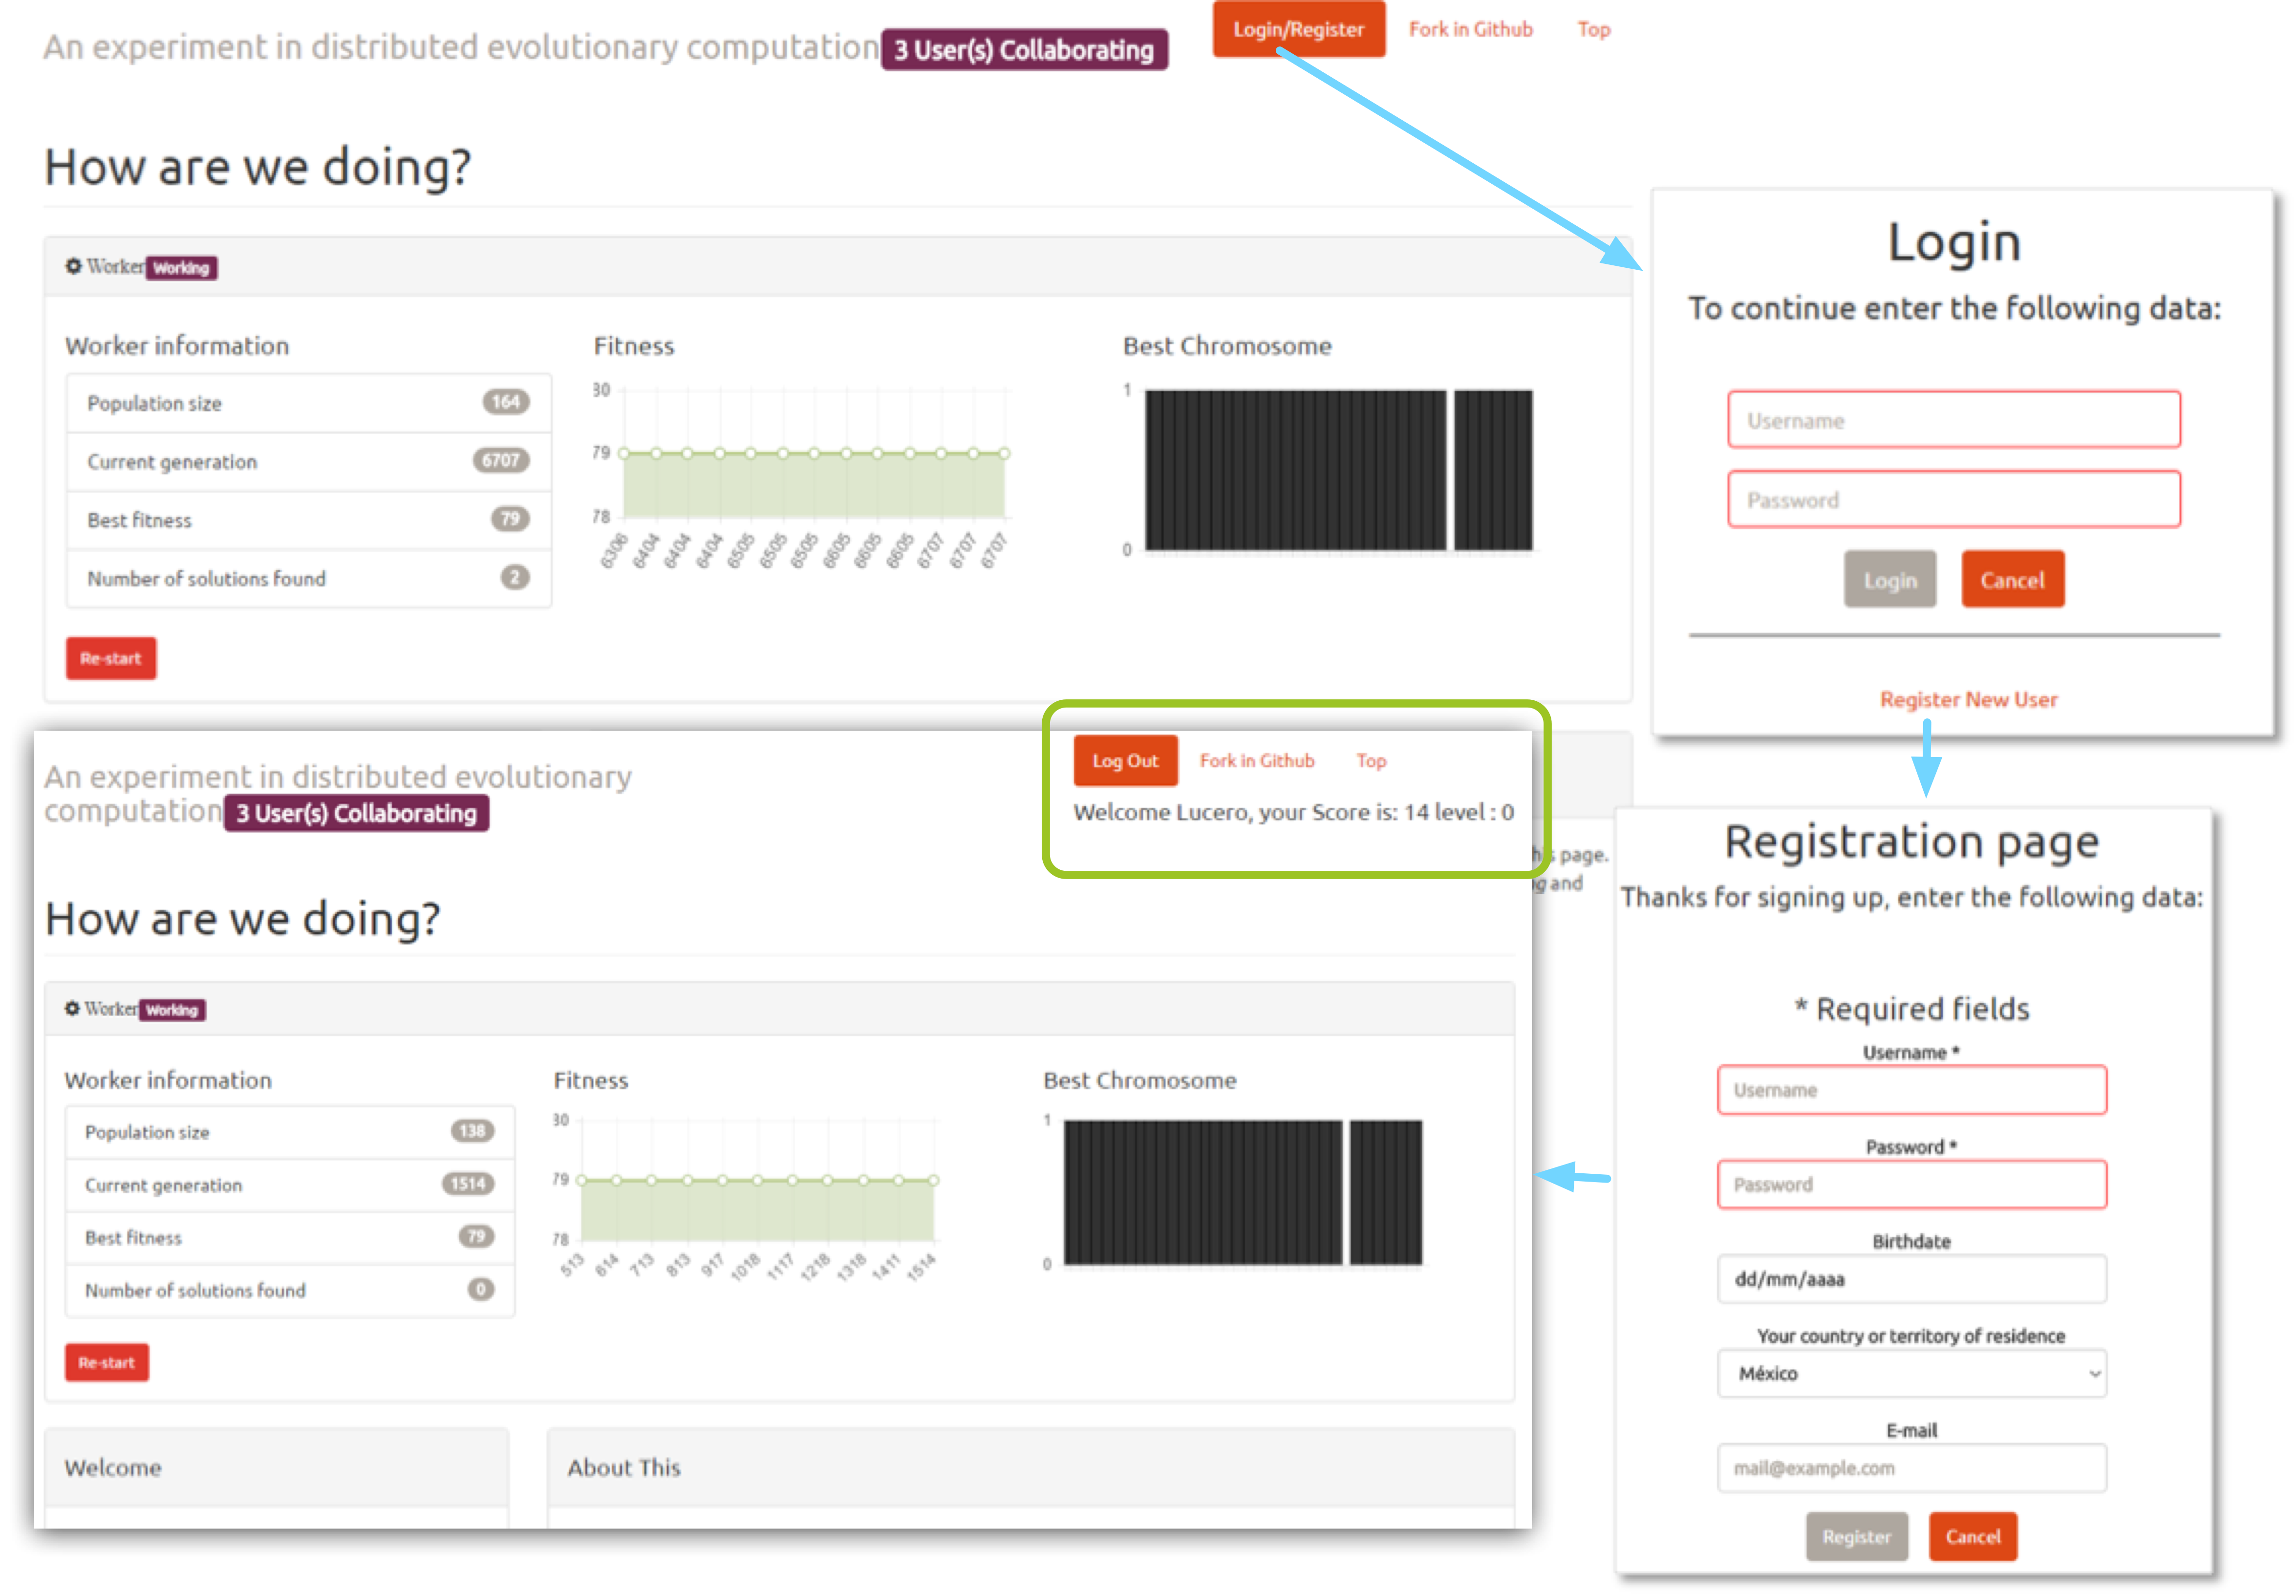
\includegraphics[width=5in]{img/login.png}
    \caption{Comparison of 30 runs of the 128 Bit OneMax problem. 
    Box-plot of the number of evaluations needed for solution, with a 2, 6 and 12 workers
    homogeneous configuration on the left side, and Heterogeneous configuration on the
    right side of each.
    }
    \label{fig:comp-onemax}
\end{figure*}

\section{Related Work}
\label{sec:experiments}
In volunteer distributed computing the BOINC projects applies a gamification technique 
by having a web page to present the ``Top 100 multi-project BOINC participants'' where
the name of the volunteer, the number of projects, GFLOPS, country and team are presented 
(\url{https://boinc.berkeley.edu/chart_list.php}). 


\section{Gamification Technique}
\label{sec:experiments}
A definition given by Huotari  \cite{huotari2012defining} is ``Gamification is
the process by which gaming concepts are brought to the real world tasks associated with
real people''. Gamification uses game design elements out of the domain of games 
with the objective of enhancing the user's experience, engagement, productivity, 
learning, among others. Deterding et al. proposes the following definition:
 ``Gamification” is the use of game design elements in non-game contexts'' 
 \cite{deterding2011gamification}.

Gamification techniques in a volunteer context seeks to persuade 
users to use their natural desire to compete, learn and socialize in 
given non-game context application \cite{deterding2011game, hamari2014does}.  
Some works give a form of reward to users, these include 
points \cite{sutter2010browse}, achievement badges or levels \cite{hamari2011framework}, 
the filling of a progress bar \cite{o2010get}, or providing the user with virtual currency.
By Making the rewards for  tasks achievements visible to other players or 
providing leader boards are ways of encouraging players to compete \cite{hickman2010total}. 
Competitio can also have problematic consequences, which can result in
negative conduct, low cooperation and collaboration, or disadvantaging certain player demographics
such as women \cite{kumar2013gamification}. Another techniques to gamification 
is to make existing tasks feel more like games \cite{deterding2010just}. 
Some techniques used in this approach include adding meaningful choice, 
onboarding with a tutorial, increasing challenge, and adding narrative \cite{mcgonigal2011reality}.




\section{Experiment}
\label{sec:experiments}
In the browser, each page visiting the experiment loads an HTML Worker
that runs a local island of an evolutionary algorithm to solve a
multimodal problem called {\em l-trap}, which has been used extensively 
as a benchmark for evolutionary algorithms \cite{fernandes2009using,nijssen2003analysis}. 
This function counts the number of bits in a sequence $l$ and assigns
the local maximum $a$ if it has got 0 bits and the global maximum $b$ if it has $l$
bits. As seen in Figure \ref{fig:trap} the fitness falls into a {\em trap} 
as the number of bits is increased, decreasing linearly until a change in slope 
is reached at point $z$, adding deceptive component for evolutionary algorithms. 
To increase the difficulty trap functions can be concatenated.
In our case we have used $40$ concatenated traps. The trap function  defined as:   
\[ f(u)= 
    \begin{cases} 
      \frac{a}{z}(z-u) & \text{if } u\leq z\\
      \frac{b}{l-z} (u-z)& \text{otherwise} 
   \end{cases}
\]
\begin{figure*}[t]
    \centering
        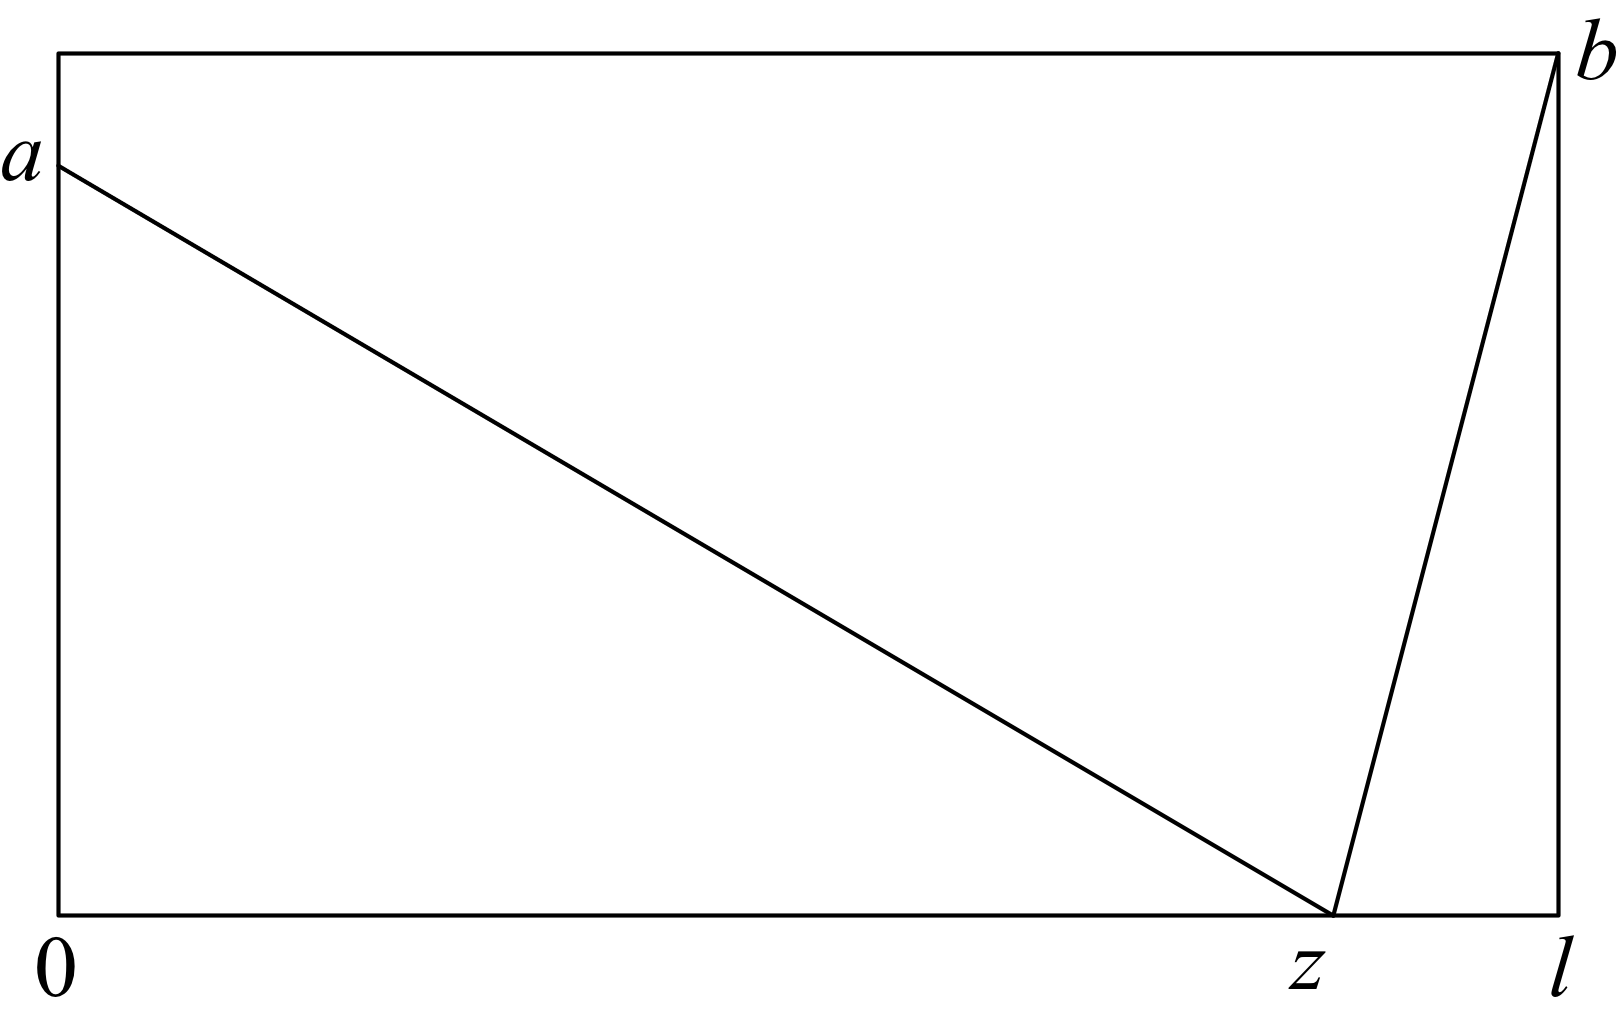
\includegraphics[width=3in]{img/trap.png}
    \caption{Trap function.
    }
    \label{fig:trap}
\end{figure*}

Each local GA had the following parameters, the initial population was randomly generated 
with sizes between 128 and 256 individuals, the period to send individuals to the server
was set at 100 local generations, the parameters for the trap function are $l$ = 4 and $b$ = 2.



\subsection{Results}
\label{sec:results}

\begin{figure*}[t]
    \centering
    \subfigure  [6 workers]
    {
        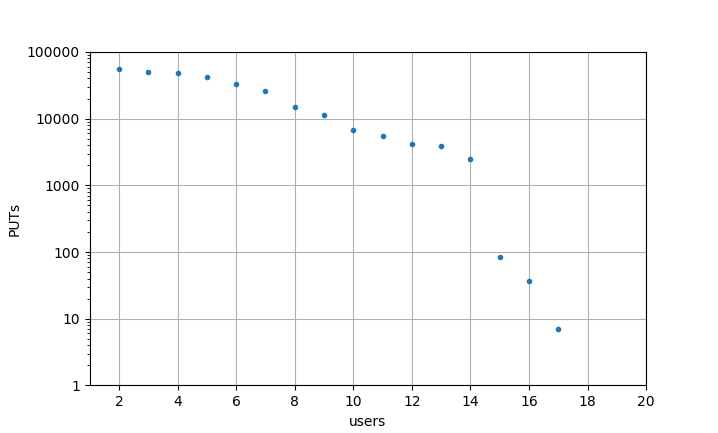
\includegraphics[width=4in]{img/puts_user.png}
    }
    \subfigure  [12 workers]
    {
        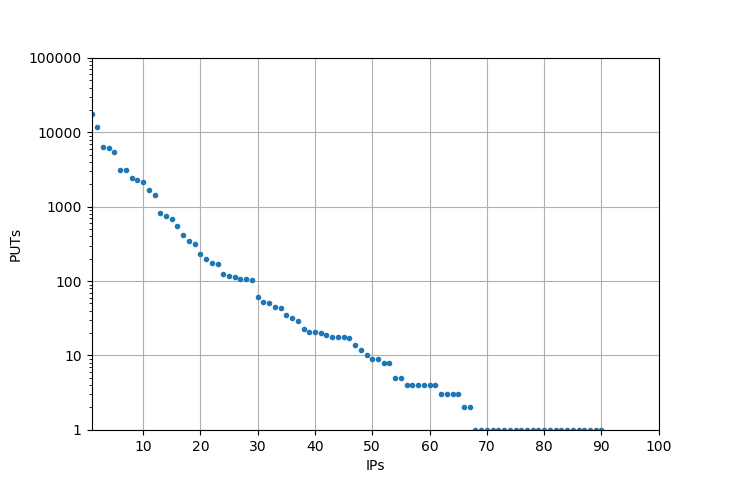
\includegraphics[width=4in]{img/puts_ip.png}
    }

    \caption{100 experiments with random parameters for the 128 Bit Griewank 
    single-objective optimization test function. Experiments are ranked by 
    the mean time to solution of 5 runs, with (a) 6 workers, and (b) 12 workers.}
    \label{fig:griewank}
\end{figure*}


\begin{figure*}[t]
    \centering
        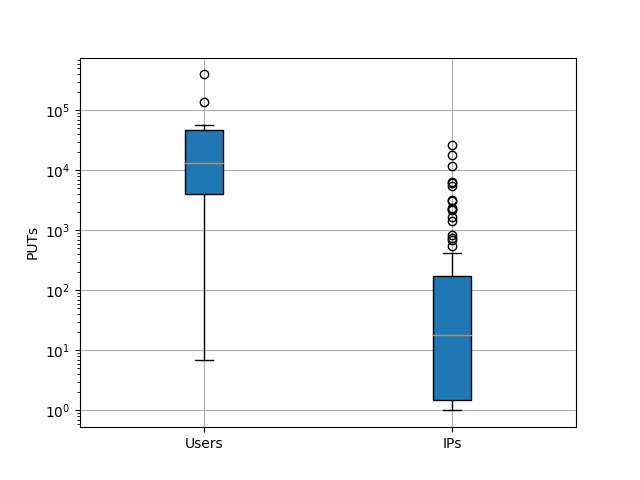
\includegraphics[width=4in]{img/puts_box.png}
    \caption{Comparison of 30 runs of the 128 Bit OneMax problem. 
    Box-plot of the number of evaluations needed for solution, with a 2, 6 and 12 workers
    homogeneous configuration on the left side, and Heterogeneous configuration on the
    right side of each.
    }
    \label{fig:comp-onemax}
\end{figure*}

\begin{figure*}[t]
    \centering
        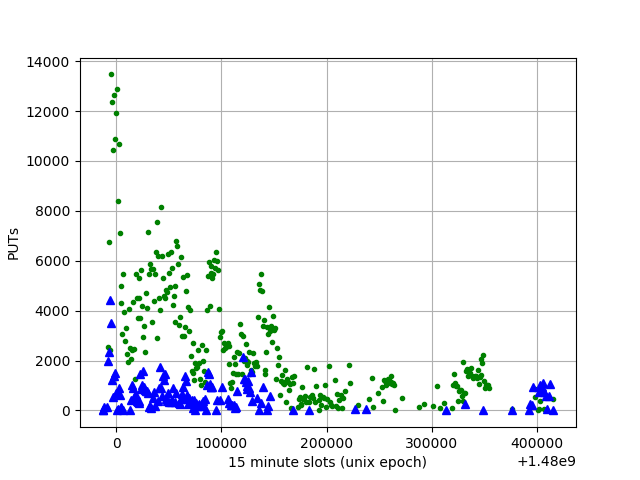
\includegraphics[width=5in]{img/puts_by_time.png}
    \caption{Comparison of 30 runs of the 128 Bit OneMax problem. 
    Box-plot of the number of evaluations needed for solution, with a 2, 6 and 12 workers
    homogeneous configuration on the left side, and Heterogeneous configuration on the
    right side of each.
    }
    \label{fig:comp-onemax}
\end{figure*}
\begin{figure*}[t]
    \centering
        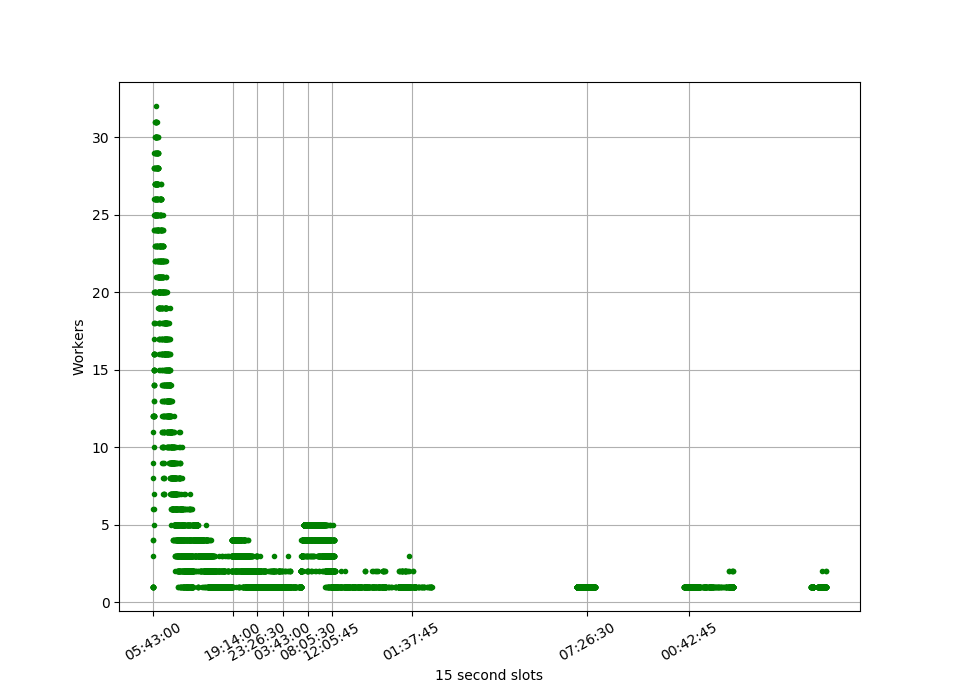
\includegraphics[width=5in]{img/workers_best_user.png}
    \caption{Comparison of 30 runs of the 128 Bit OneMax problem. 
    Box-plot of the number of evaluations needed for solution, with a 2, 6 and 12 workers
    homogeneous configuration on the left side, and Heterogeneous configuration on the
    right side of each.
    }
    \label{fig:comp-onemax}
\end{figure*}
\begin{figure*}[t]
    \centering
        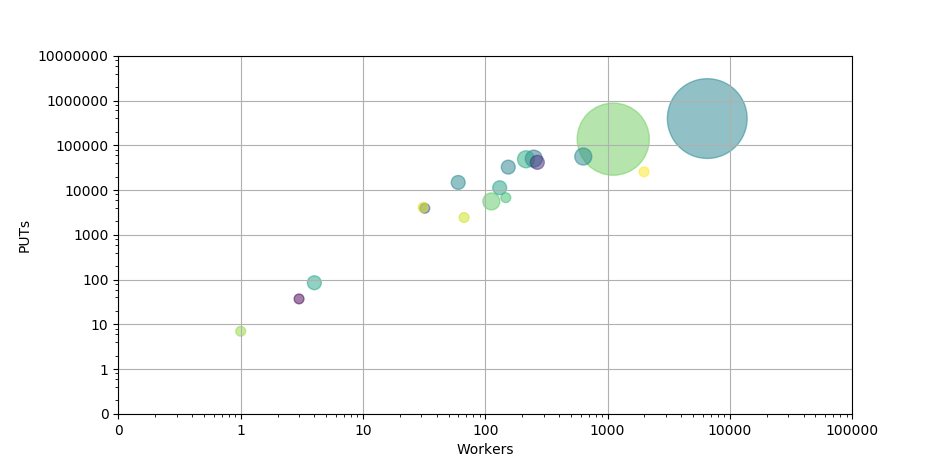
\includegraphics[width=5in]{img/workers_put_ip.png}
    \caption{Comparison of 30 runs of the 128 Bit OneMax problem. 
    Box-plot of the number of evaluations needed for solution, with a 2, 6 and 12 workers
    homogeneous configuration on the left side, and Heterogeneous configuration on the
    right side of each.
    }
    \label{fig:comp-onemax}
\end{figure*}

\bibliographystyle{abbrv}
\bibliography{../../bib/biblio,../../bib/evospace-i,../../bib/volunteer,../../bib/geneura}
\end{document}
